% This must be in the first 5 lines to tell arXiv to use pdfLaTeX, which is strongly recommended.
\pdfoutput=1
% In particular, the hyperref package requires pdfLaTeX in order to break URLs across lines.

\documentclass[11pt]{article}

% Remove the "review" option to generate the final version.
\usepackage{ACL2023}

% Standard package includes
\usepackage{times}
\usepackage{latexsym}

% For proper rendering and hyphenation of words containing Latin characters (including in bib files)
\usepackage[T1]{fontenc}
% For Vietnamese characters
% \usepackage[T5]{fontenc}
% See https://www.latex-project.org/help/documentation/encguide.pdf for other character sets

% This assumes your files are encoded as UTF8
\usepackage[utf8]{inputenc}

% This is not strictly necessary, and may be commented out.
% However, it will improve the layout of the manuscript,
% and will typically save some space.
\usepackage{microtype}

% This is also not strictly necessary, and may be commented out.
% However, it will improve the aesthetics of text in
% the typewriter font.
\usepackage{inconsolata}

% newly added
\usepackage{multirow}
\usepackage{graphicx}
\usepackage{stfloats}
\usepackage{subfigure}

\newcommand{\tabincell}[2]{\begin{tabular}{@{}#1@{}}#2\end{tabular}}
\newcommand{\secref}[1]{Section \ref{#1}}
\newcommand{\figref}[1]{Figure \ref{#1}}
\newcommand{\eqnref}[1]{Eq. (\ref{#1})}
\newcommand{\tabref}[1]{Table \ref{#1}}
\newcommand{\exref}[1]{Example \ref{#1}}
\newcommand{\KZ}[1]{\textcolor{blue}{(Kenny: #1)}}
\newcommand{\MY}[1]{\textcolor{red}{(Mengyue: #1)}}
\newcommand{\JY}[1]{\textcolor{orange}{(Jieyi: #1)}}
\newcommand{\CH}[1]{\textcolor{green}{(Chunhao: #1)}}

% If the title and author information does not fit in the area allocated, uncomment the following
%
%\setlength\titlebox{<dim>}
%
% and set <dim> to something 5cm or larger.

\title{Transcribing Vocal Communications of Domestic Shiba lnu Dogs}

% Author information can be set in various styles:
% For several authors from the same institution:
% \author{Author 1 \and ... \and Author n \\
%         Address line \\ ... \\ Address line}
% if the names do not fit well on one line use
%         Author 1 \\ {\bf Author 2} \\ ... \\ {\bf Author n} \\
% For authors from different institutions:
% \author{Author 1 \\ Address line \\  ... \\ Address line
%         \And  ... \And
%         Author n \\ Address line \\ ... \\ Address line}
% To start a seperate ``row'' of authors use \AND, as in
% \author{Author 1 \\ Address line \\  ... \\ Address line
%         \AND
%         Author 2 \\ Address line \\ ... \\ Address line \And
%         Author 3 \\ Address line \\ ... \\ Address line}

\author{Jieyi Huang$^1$, Chunhao Zhang$^2$, Mengyue Wu$^{3*}$, 
Kenny Q. Zhu$^4$\thanks{\hspace{2mm}Corresponding authors.}\\
	$^{1,2,3,4}$Shanghai Jiao Tong University, Shanghai, China \\
	% Affiliation / Address line 3 \\
	\texttt{$^1$xsiling1@gmail.com}, 
	\texttt{$^2$forest\_zch@sjtu.edu.cn}\\ 
	\texttt{$^3$wumengyue@cs.sjtu.edu.cn}, 
	\texttt{$^4$kzhu@cs.sjtu.edu.cn}\\}
\begin{document}
\maketitle
\begin{abstract}
How animals communicate and whether they have languages is a persistent
curiosity of human beings. However, the study of animal communications
has been largely restricted to data from field recordings or in a controlled
environment, which is expensive and limited in scale and variety. %thus statistically insignificance. 
%People hold intense interest to learn what animals are expressing for 
%research, related applications, or sometimes just curiosity. 
In this paper, we take domestic Shiba Inu dogs as an example and
extract their vocal communications from a large amount of
YouTube videos of Shiba Inu dogs. We classify these clips into different scenarios and locations, and further transcribe
the audio into phonetically symbolic scripts through a systematic
process. We discover consistent phonetic symbols among their expressions, which indicates that Shiba Inu dogs can have systematic verbal communication patterns. This reusable framework produces the first-of-its-kind Shiba Inu
vocal communication dataset that will be valuable to future research
in both zoology and linguistics. 
%\MY{Add ``Consistent phonetic symbols are discovered from these dogs indicating that they have systematic verbal communication patterns''?}
 
%For dogs, which are one of the most common animals around humans, many researchers have tried to know their meanings of voice. However, these previous researches most took dogs’ voice as an entirety and ignored the internal patterns. At the same time, these datasets used were in limited scenes and sizes which lacked universality. In this paper, we have gained phoneme-grid Shiba Inu dogs audios from open public media through a reusable systematic process and assigned phoneme labels like International Phonetic Alphabet through clustering. Finally, a large-size audios with transcripts dataset of Shiba Inu dogs is constructed, which will facilitate further research in this area.
\end{abstract}

% \section{Introduction}

% These instructions are for authors submitting papers to ACL 2023 using \LaTeX. They are not self-contained. All authors must follow the general instructions for *ACL proceedings,\footnote{\url{http://acl-org.github.io/ACLPUB/formatting.html}} as well as guidelines set forth in the ACL 2023 call for papers.\footnote{\url{https://2023.aclweb.org/calls/main_conference/}} This document contains additional instructions for the \LaTeX{} style files.
% The templates include the \LaTeX{} source of this document (\texttt{acl2023.tex}),
% the \LaTeX{} style file used to format it (\texttt{acl2023.sty}),
% an ACL bibliography style (\texttt{acl\_natbib.bst}),
% an example bibliography (\texttt{custom.bib}),
% and the bibliography for the ACL Anthology (\texttt{anthology.bib}).
\section{Introduction}

Protein$-$protein interactions (PPIs) are of central importance for the majority of biological functions, such as signal transduction, metabolic pathways, molecular dynamics, and protein networks\cite{Hoffmann.Krallinger.ea:2005}, for they serve as the most fundamental building blocks of the entire interacademic systems of any organisms. Collecting data on pairwise interaction relationships is essential for multiple purpose, including identification of modules with certain functionality\cite{Spirin.Mirny.03}, mapping diseases to dominated genes\cite{Ideker.Sharan.08}, and after all, understanding wholistic metabolic/genetic networks from a system biology perspective.

A lot of databases have been built to store protein and genetic interactions from major model organism species and are available in various standardized formats, such as MINT\cite{Zanzoni.Montecchi-Palazzi.ea:2002}, BIND\cite{Bader.ea:2003}, BIOGRID\cite{DBLP:journals/nar/StarkBRBBT06}, etc. Among those mainstream databases, the data largely rely on voluntary reports by scientists or researchers, besides, comprehensive curation efforts become indispensable for the sake of accuracy. However, the amount of biology-related literatures with respect to protein interactions grows explosively and thus make it either impossible or impractical to manually detect PPI information anymore.

Considering huge amount of PPI information with great wealth hidden in published papers, in recent years, numerous mining techniques have been proposed that aim to extract PPI information automatically from free text, especially machine learning, information retrieval, and natural language processing\cite{DBLP:journals/bib/WinnenburgWPDS08}.These approaches can be roughly categorized into three classes: co$-$occurrence, rule$-$based, and machine learning. 

Co$-$occurrence is the approach with most simplicity and naivete. Just as its name implies, this method intends to find out pairs of proteins that co-occur in the same context. The scope of "same context" ranges from phrase, sentence, paragraph to whole abstract, even document. The underlying assumption is that whenever two proteins are mentioned together by authors, chances are high that there is some kind of relationship between them. However, however, in-context closeness even semantic relation does not necessarily represent actual biological interaction. As a consequence, a large fraction of candidate pairs are mismatched inevitably, causing a high recall but low precision.

The second approach is rule-based extraction, in other words, pattern matching. There are many types of rules, most of them concern natural language processing (NLP). One way is to specify hand-crafted regular expressions before hand, which mostly lean on language usage preference. Besides, by using full or partial (shallow) parsing strategies, more information would be acquired, such as part-of-speech taggers, local dependencies between syntactic components, context-free grammar\cite{DBLP:journals/bioinformatics/TemkinG03}, and full sentence structure. Compared to co$-$occurrence, rule-based approach enjoy better precision but much lower recall. In addition, since the rules are usually derived from training data, that is to say, the improper choice of training data would be significantly lethal, therefore quality of extraction is invariably instable and may not applicable to other data.

The third and most commonly used approach use machine learning techniques, in this case, the task to extract protein$-$protein interactions turns out to be a binary classification problem. Each protein pairs are represented along with a set of features, which is associated with their context, then a well$-$defined classifier gives the answer whether the candidate protein pairs is classified to be qualified PPI. (TO BE FURTHER FILLED!!!)

In this paper, we introduce a general bootstrapping framework for Protein$-$protein interaction extraction from natural text.Our method differs from most of the previous works in three aspects:

(1)The extraction process is driven by only tiny fraction of training data, which are regarded as seed data. In each round, it would derive reliable patterns automatically from seed data, then extract more positive PPI pairs consequently, what's more, the seed data would be augmented by the newly extracted results with high confidence.

(2)multiple graph kernel. 

(3)various evaluation.




\section{Approach}
\label{sec:approach}
In this section, we first introduce the general framework of ChatMatch, which is modeled as
a sport tournament, then discuss some possible scoring functions that can be used by
the virtual judges in these competitions.

%Our whole evaluation framework consists of competition and scoring at three different levels. 
%The game level is at the bottom 
%and is played between two players. 
%Then comes the match level.
%To ensure the fairness of the game, 
%two games will be played between every two robots, 
%with each side starting a conversation.
%The result of two games determines the outcome of a match. 
%The tournament level is at the top
% and is composed of matches among different pairs of players. 

\subsection{Competition Protocol}
\label{sec:competition}
The competition takes place, from top to bottom, at tournament, match and
game levels.

\subsection*{Tournament Rules}
%\KZ{Give an overview of the how the tournament is run.}
We adopt a double round-robin 
sports tournament, where all bots participating in the competition 
converse directly with each other twice.
This is better than a knock-out system because it assesses a bot's ability to
deal with both strong and weak bots.
%For example, whether with weaker bots will induce them to make more mistakes or  how stronger bots will motivate their performance.
If we have $n$ chatbots players in our tournament, 
there will be $n\times (n-1) $ games in total.

\subsection*{Match Rules}
%\KZ{Talk about how the matches are administered. Just the procedure only.}
There are two chatbots competing in a single match. 
Each match consists of two games,
 started by a different bot. 
If we have $n$ bots in our tournaments, there 
will be ${n \choose 2}$ matches in total. 

\subsection*{Game Rules}
%\KZ{The procedure of the game. How each game is started and stopped.}
Each game is started by a player whose first utterance is provided by 
the system. The choice of the first utterance can be different 
depending on the domain of the bots and the ability we want to 
rank about the bots. For example, if we want to test 
the ability on movies, we can set a movie-related 
first utterance. 

During a game, there might be different ways to 
end the conversation. We can set a fixed number of exchanges 
or a terminating condition such as whether a bot makes a fatal error
or whether a certain score is reached.

\begin{table*}[th]
\centering
\scriptsize
\begin{tabular}{c|l|l}
%\hline
\toprule
\textbf{Dimension} & \textbf{Definition} &\textbf{Approach} \\ \midrule
Fluency  & Responses are fluent and natural.& Sentence perplexity. \\
Knowledge & Responses indicate the bot has the knowledge. & The number of times the bot expresses its ignorance to a question.\\
Proactivity & Responses actively proceed the conversation.&The number of times the bot raises a question. \\
Specificity & Responses are not generic.&The average of Distinct-1 and Distinct-2 \citep{li2015diversity}.\\
Diversity &Responses which are diverse and non-repetitive. &Repetition detection following the function in \algoref{algo:rep}. \\
Consistency &Responses do not contradict chat history. &Detect inconsistent questions following the function in \algoref{algo:inconsist}\\
Relevance & Responses are related to current context.& Ability to catch the relevant concept in chat history defined in \algoref{algo:bonus}. \\
\bottomrule
\end{tabular}
\caption{Seven evaluation dimensions.}
\label{tab:methods}
\end{table*}


\subsection{Scoring}
\label{sec:scoring}
\subsection*{Game-level Scoring}
%\KZ{Define a few functions: one to catch repeating, one to chat contradiction and one to catch long term memory.}

%Here we define the rules for recording points in one game between two bots. 
Inspired by \citet{finch2020towards}, 
we score each turn based on seven aspects of rules 
concerning \textit{consistency}, \textit{fluency}, \textit{knowledge}, \textit{specificity}, 
\textit{diversity}, \textit{relevance} and \textit{proactivity}. 
%As these seven metrics present a high level of 
%overlap among all distinct evaluation metrics used 
%during different process of human evaluation,
%we believe the combination of these seven distinct dimensions will be reliable. 
Finally, we sum up the scores for each bot for all the turns.
\tabref{tab:methods} documents the definition of these dimensions, which can all be scored
automatically.

%After finishing the calculation of the bonus and penalty scores for each turn, we obtain the scores of the two bots in a game with weighted sum according to \eqnref{eq:sum-up}

%\begin{equation}
%S(bot) = \sum_t - c\times C(t)  - r \times R(t) + b \times B(t)
%\label{eq:sum-up}
%\end{equation}
%$S$ denotes the total score gained by a bot for a game.
\begin{figure}[th]
        \centering
        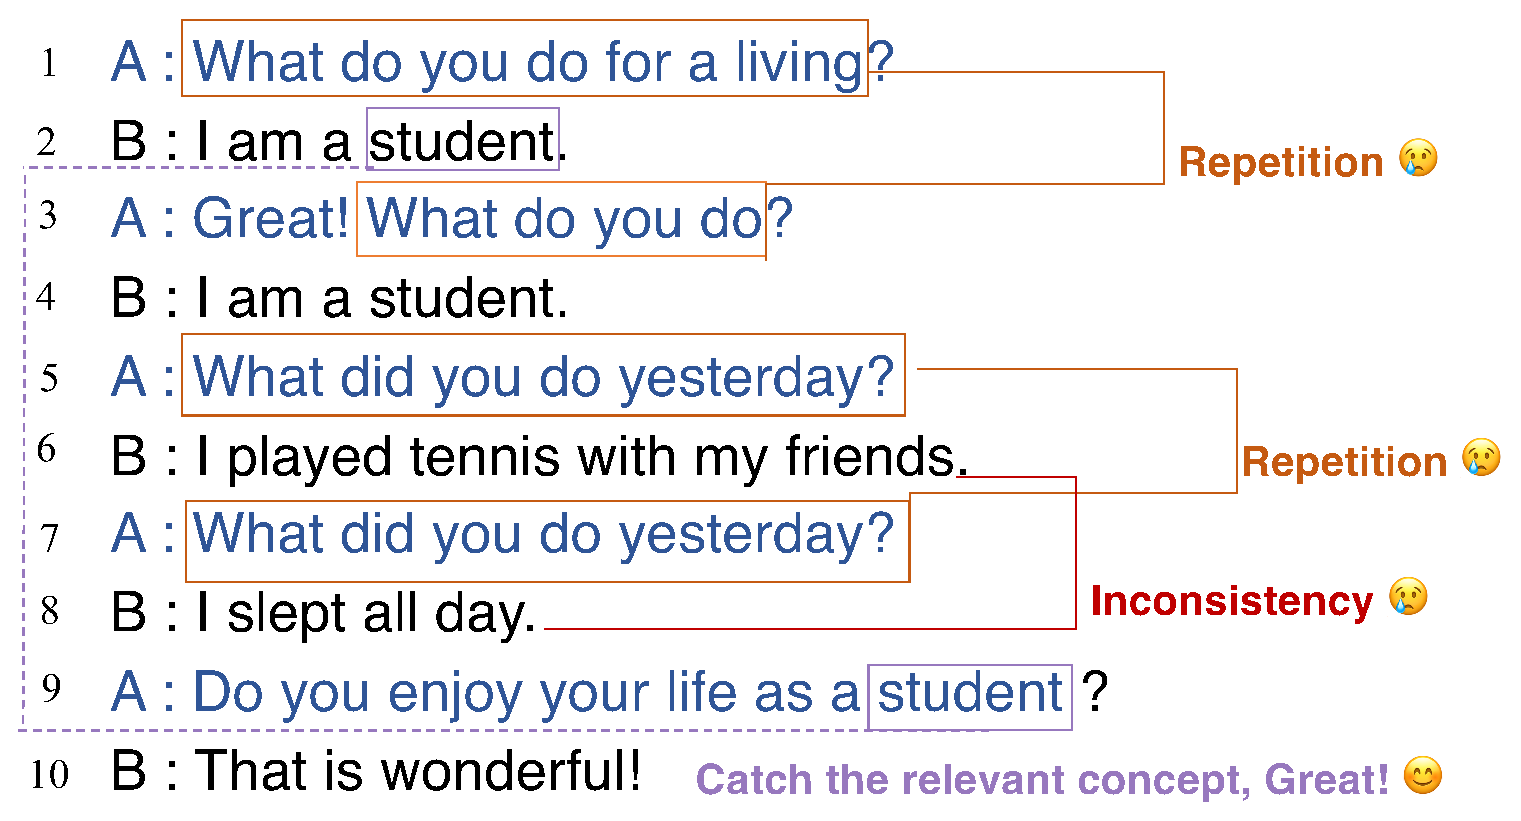
\includegraphics[width=0.95\columnwidth]{example2.eps}
        \caption{A chat snippet between two bots.}
        \label{fig:example}
\end{figure}

Fluency, Knowledge, Proactivity and Specificity are scored for each turn separately
and aggregated at the end of the conversation.
Detection for diversity, consistency and relevance are more involved and are explained
using \figref{fig:example}. 

As for diversity, at each turn $t$, we first check if there exists any repetitive question.  
We can easily find turn 3 and turn 7 repeated turn 1 and turn 5 
respectively. They will then be penalized one point for repetition. 
Repetition is not penalized if the previous turn is already 
marked as a repetitive question. For example, in \figref{fig:example}, 
although turn 4 is considered a repetition of turn 2,  
we are not going to penalize it as turn 3 is a repetitive question. 

The detection of inconsistency is always triggered after the detection of repeated questions. 
If the answers to the same questions are different, we will penalize the current turn, 
such as turn 8 in \figref{fig:example}.

We decide a repetition or an inconsistency by calculating the similarity of the two turns. 
We use a similarity function to complete the calculations, which we will 
discuss in \secref{sec:experiment}. The actual diversity and consistency scores
are the negation from the amount of repetition and inconsistency.

Relevance is assessed as a bonus to reward
a bot if it is able to memorize the important relevant concepts that have shown up 
before in the conversation. We sort the concepts that have shown up in 
chat history by their IDF scores. For example, in turn 9, $A$ 
mentions the concept word ``student'' presented by $B$ in turn 2. With this
turn, $A$ will win a bonus point.


The algorithms and notations for computing diviersty, consistency and relevance are included
in \tabref{tab:functions}, \algoref{algo:rep}, \algoref{algo:inconsist}, and \algoref{algo:bonus}. 

\begin{table}[th]
\centering
\small
\begin{tabular}{c|l}
%\hline
\toprule
\textbf{Notation} & \textbf{Description} \\ \midrule
$t$ & Current turn \\
$H(t)$  &  a list of history turns prior to $t$ \\
$Sim(x,y)$ & similarity between two turns $x$ and $y$ \\
$\sigma_r$ & Threshold for detecting repetition \\
$\sigma_c$ & Threshold for detecting consistency \\
$r$ & Weight for repetition \\
$c$ & Weight for inconsistency \\
$b$ & Weight for bonus \\
$d$ & Min distance between consecutive mentions \\
IDF list & List of lemma in chatlog sorted by IDF\\
$p$ & Percentage of important lemmas in IDF list\\
$R(t)$ &  Repetition penalty for turn $t$ \\
$C(t)$ &  Inconsistency penalty for turn $t$ \\ 
$B(t)$ &  Memory bonus for turn $t$ \\
$Rep(t)$ & A list of repeated turns for turn $t$ \\  
\bottomrule
\end{tabular}
\caption{
Functions and variables in algorithms.}
\label{tab:functions}
\end{table}

\begin{algorithm}[th]
\small
\caption{Scoring for Diversity}
\label{algo:rep}
\hspace*{0.02in} {\bf Input:}
 $t$, $H$, $Sim$, $\sigma_{r}$
; \hspace*{0.02in} {\bf Output: } 
 $R$;
\begin{algorithmic}[1]
\State //Starting to detect repetition
\For {$u$ in $H(t)$}
	\If {$Sim(t,u) \geq \sigma_{r}$}
		\State Add $u$ to $Rep(t)$
	\EndIf
\EndFor
    \If{$len(Rep(t))\geq 0$}
        \If{$t$ is a question and We can find a question in $Rep(t)$}
        \State $ R(t) \leftarrow  R(t) + 1$ 
        \Else
        \If {the previous turn of $t$ is not a repetitive question}
        \State $R(t)) \leftarrow R(t) + 1$ 
        \EndIf
        \EndIf
    \EndIf
\end{algorithmic}
\end{algorithm}


\begin{algorithm}[th]
\small
\caption{Scoring for Consistency}
\label{algo:inconsist}
\hspace*{0.02in} {\bf Input:}
$t$, $H$, $Sim$, $\sigma_{c}$
; \hspace*{0.02in} {\bf Output:  } 
 $C$;
\begin{algorithmic}[1]
\State // Inconsistency detection
 \If {previous turn of $p$ is a repetitive question} 
   \If{ the response $res$ to the question repeated by turn $p$ contradicts turn $i$ with $Sim(t, res) \leq \sigma_{c}$ }
    \State $C(t) \leftarrow C(t) + 1$
   \EndIf
  \EndIf
\end{algorithmic}
\end{algorithm}

\begin{algorithm}[th]
\small
\caption{Scoring for Relevance}
\label{algo:bonus}
\hspace*{0.02in} {\bf Input:}
$t$, $p$, $d$
; \hspace*{0.02in} {\bf Output:  } 
$B$;
\begin{algorithmic}[1]
\State // Assessing the ability of catching relevant concepts\\
$B(t) \leftarrow 0$
\For {all tokens $tk$ in current turn $t$}
 \If {$t$ - previous occurrence turn of $tk > d$ and $tk$ in the top $p\%$ of the IDF list of all tokens in the dialogue} 
   \State $B(t) \leftarrow 1$
  \EndIf
 \EndFor
\end{algorithmic}
\end{algorithm}

At the end of each game, each bot gets seven scores, one for each dimension.  
After pairwise comparison on individual dimension, a bot gains one point for win and zero point for a tie or lose.
The final score of each bot is determined by the sum of their individual scores.
%\KZ{Are these scores positive or negative? Comparable between bots?}

\subsubsection*{Match-level Scoring}
%\KZ{Use an equation to compute the final scores?}
One match which consists of two games, each started with a different bot, 
decides winning or losing between two bots.
For match-level scoring, we mimic the scoring rules of soccer tournament. 
For each match, $W$ points for the winner,  
$T$ points for a tie and 
$L$ points for the loser.
The value of $W$, $T$ and $L$ will be discussed in \secref{sec:ablation}. 

%\KZ{At the match level, we need to consider different starting context for the bots? I think we should present a few options for the reader and say that we are limited to these.}

\subsubsection*{Tournament-level Scoring}
%\KZ{Use an equation to compute the final scores?}
We count the points by simply summing up their scores gained in every match. Currently, several bots with the same final rank are tolerated. For future study, it's possible to mimic more detailed rules presented in sports match such as determine their ranking based on their win-loss relationship in the match between them.  
If they are still tied, we could propose an “overtime” for these two bots, one human judge may observe their performance and then make the decision of the game.

\subsection{Dataset}
\label{sec:data}
To train and evaluate our approach of detecting false rumors, a labeled
data set is needed.
We collect a set of known false rumors from Sina community management center \cite{website:Manage},
which deals with reporting
of issues including various misinformation which we regard as
certified false rumors.
% consists of all kinds of fields, so the diversity of rumors is guaranteed.
There are 11466 reported false rumors between 2012/05/28 and 2014/04/11.
%in the result publication category at that time excluding the those without links for the original message webpages.
%Above rumor data are captured directly from Sina Weibo's mobile website.
Since a rumor must have sufficient circulation, we only keep those false
rumors that have at least 100 reposts, which leaves us with 2601 false rumors
up to 2014/04/11.
%and all their reposting information by the time of being captured excluding abnormal original message links.
%Some previous works \cite{yang2012automatic} also made use of
%Sina Weibo's official acount to collect false rumors.
%But at that time, Sina Weibo had not constructed the community management
%and there was an only official false rumor busting account in
%Sina Weibo posting some identified misinformation to public.
%One problem is that the false rumor reports posted by the account
%had no links to the original messages so they needed to
%construct queries manually to find out the original messages.
Sina Weibo API provides interfaces to capture the information of
original messages as well as their repost messages.
From Sina Weibo API, we captured the post time, post client
and content of 2601 false rumors along with all their reposts.

In the real world, the number of false rumors on Sina Weibo
is much smaller than the number of normal messages (1 out of 9 or less).
Thus a ``dummy'' classifier that rules all messages as normal messages
will achieve a very high accuracy (above 90\%) on real-world data.
To avoid this problem, we construct a data set with roughly equal number of
false rumors and normal messages. Most studies in the past also use
data sets which are either 50-50 split
\cite{castillo2011information,jin2013epidemiological}
or close to that \cite{yang2012automatic,qazvinian2011rumor}.
Thus, we randomly select 5000 other Weibo original messages
which are not proved to be false as well as their reposts
using the Sina Weibo API. Then, we manually filtered out messages with fewer than 100 reposts as well as false rumors to form a set of 2536 normal messages.
%To make non-rumors be in accord with rumors, we also only select the tweets that have 100 reposts at least here. The profiles of users involved are included in the data captured from API. Afterwards, we labeled 2844 pieces of non-rumors from them manually.
Each message or repost contains links to the author profile
information such as age, gender, number of followers and friends,
and can be crawled using the Weibo API.
%
%Sina Weibo provides API to capture a user's information but the speed is too slow because of frequency restriction. So we capture the original poster's information through Sina Weibo API and the other users' information directly from their homepages on Sine Weibo's mobile website.
%

At the end of this phase, our labeled data set 
\footnote{The labeled data set of the original messages (without reposts)
is available at \url{http://adapt.seiee.sjtu.edu.cn/~kzhu/rumor/}.}
consists of 2601 false rumors, 2536 normal messages
and with 4 million distinct users involved in these messages. Of these
500 false rumors and 500 other messages (called small data set) are used for
SVM parameter tuning while
the rest (called big data set) are used for end-to-end cross validation.

\section{Analysis}

We present preliminary statistical findings from ShibaScript, including lexical analysis and transcribing accuracy evaluation.
% \KZ{rewrite this preamble, it's irrelevant now: To give a detailed picture about our dataset ShibaScript and also show several statistical syntax results on it, we will explain our analysis below.}

% This is the analysis on this dataset. Inlcuding its distribution and some further analysis inlcuding bigrams.

% \subsection{Source Information}
% \label{sec:sourceinformation}
% The 16 dogs come from 16 different Japanese user accounts at YouTube. From the videos uploaded from the specific user and the captions attached to these videos, we can get to know much about the growing up environments of dogs, which will influence the expressions of these dogs to some degree. %The environments of them are in \ref{tab:sourceinformation}.
%这是狗的来源的信息,包含地区、是否家养、之类的

% \begin{table}[th]
% \centering
% \begin{tabular}{c|c|c|c}
% \hline
% \textbf{Dog Index} & \textbf{Color} & \textbf{Other Pets} & \textbf{Area}\\\hline
% 0 & yellow & \\
% 1 & yellow & \\
% 2 & yellow & \\
% 3 & yellow & \\
% 4 & yellow & \\
% 5 & yellow & \\
% 6 & yellow & \\
% 7 & yellow & \\
% 8 & yellow & \\
% 9 & yellow & True \\
% 10 & yellow & \\
% 11 & yellow & \\
% 12 & yellow & \\
% 13 & yellow & \\
% 14 & yellow & \\
% 15 & black & \\\hline
% \end{tabular}
% \caption{The source information of dogs in ShibaScript. Color means the fur color of the dog. Other Pets means whether the dog is kept with a family with other animals. Area means the living locations of the family.}
% \label{tab:sourceinformation}
% \end{table}



% \begin{table}
% \centering
% \begin{tabular}{c|c|c|c|c}
% \hline
% \multirow{2}{*}{\textbf{DogID}} & \multicolumn{2}{c|}{\textbf{Sentence}} & \multicolumn{2}{c}{\textbf{Word}}  \\
% \cline{2-5}
% {} & \textbf{Num} & \textbf{Length(s)} & \textbf{Num} & \textbf{Length(s)} \\
% \cline{1-5}
% 0 & 346 & 1107.67 & 577 & 363.36\\
% 1 &  158 & 514.24 & 241 & 129.00\\
% 2 & 553 & 1643.00 & 847 & 469.20\\
% 3 &  55 & 171.69 & 123 & 65.52\\
% 4 & 56 & 224.00 & 107 & 94.08\\
% 5 &  115 & 374.58 & 217 & 98.52\\
% 6 & 52 & 157.00 & 77 & 47.72\\
% 7 & 40 & 135.00 & 65 & 27.44\\
% 8 &  135 & 566.03 & 316 & 143.68\\
% 9 & 255 & 795.00 & 408 & 157.08\\
% 10 & 1188 & 4306.00 & 2029 & 1372.52\\
% 11& 188 & 570.94 & 320 & 203.20\\
% 12  & 130 & 562.28 & 257 & 147.00\\
% 13  & 993 & 2930.19 & 1719 & 749.72\\
% 14  & 118 & 350.11 & 324 & 144.76\\
% 15  & 87 & 299.88 & 134 & 101.24 \\\hline
% sum & \textbf{4469} & \textbf{14707.61} & 7761 & 4314.04\\\hline
% \end{tabular}
% \caption{The basic statistical information of ShibaScript.}
% \label{tab:datasetinformation}
% \end{table}




\subsection{Lexical Analysis}
During the transcribing, there are in total 11 types of tokens, in which 9 types are phonetic symbols~(\tabref{tab:alphabet}), the other two are short pauses between words and long pauses between sentences. 

Similar to humans, the length of these tokens contain ample information. The exact lengths of tokens are kept in ShibaScript for concrete analysis. Because the long pauses are largely determined by the scene at that time, the numerical analysis of it will not be included here. 


\begin{table}[th]
\centering
\small
\begin{tabular}{c|c|c}
\hline
\textbf{Symbol} & \textbf{Mean len (s)} & \textbf{Variance (s)}\\
\hline
\verb|[au]| & 0.35 & 0.022 \\
\verb|[a]| & 0.35 & 0.017 \\
\verb|[^]| & 0.34 & 0.017\\
\verb|[u:]| & 0.45 & 0.054\\
\verb|[u]| & 0.35 & 0.030\\
\verb|[i]| & 0.33 & 0.020\\
\verb|[k]| &  0.24 & 0.009\\
\verb|[(w)au]| & 0.34 & 0.018\\
\verb|[en]| & 0.36 & 0.032\\
\verb|short pause| & 0.57 & 0.335\\
\hline
\end{tabular}
\caption{The mean and variance of the duration of 9 phonetic symbols 
and short pauses between words.}
\label{tab:tokenanalysis}
\end{table}

The mean and variance of each token length can be seen in~\tabref{tab:tokenanalysis}. In which we find that almost every phonetic symbol has a similar length of 0.35s or so. Except for the phonetic symbol \verb|[u:]|, which is a prolonged sound owning an average length of 0.45s. While phonetic symbol \verb|[k]| is a relatively short-lived symbol, only having 0.24s average length.

Considering the monogram~(\figref{fig:monogram}) of ShibaScript, we can find that the most frequent symbol is \verb|[en]|, which reaches to 3478 times in ShibaScript, the following two are \verb|[au]| and \verb|[a]|, which reaches  1981 and 2011 times respectively. One of the reasons why \verb|[en]| exceeds much, which is counterintuitive, is that symbols such as \verb|[a]|, \verb|[au]|, \verb|[(w)au]| are divided up. The least frequent symbol is \verb|[k]|, which only reaches 15 times. This is because dogs seldom produce air-sounds like \verb|[k]|.

At the same time, we can find that these phonetic symbols exist in multiple dogs' sounds, showing that these 9 symbols are universal.

\begin{figure}[th]
\centering
\scalebox{0.32}{\includegraphics{monogram.pdf}}
\caption{The occurrences of each monogram. The blue bars show the occurrences across the whole dataset of each monogram in ShibaScript, the green lines show the numbers of dogs producing the symbols, from 1 to 16.}%\KZ{Remove ``Monogram Stats'' from the pic, since
% you already talk about it in the caption.}
\label{fig:monogram}
\end{figure}

%静音片段分析
%unigram, bigram分析
After analyzing the monogram, we come to find the relationship between symbols, as well as the bigram~(\figref{fig:bigram}) of ShibaScript. Among these bigrams, several appear extremely frequently. It shows a possibility that they are associated with some common semantic meanings. We will dive into that in the future works. Due to space constraints, the detailed information of bigram is shown in~\secref{sec:appendixc}.

% 1 
\begin{figure}[th]
\centering
\scalebox{0.32}{\includegraphics{bigram.pdf}}
\caption{The occurrences of each bigram. The blue bars show the occurrences across the whole dataset of each monogram in ShibaScript, the green lines show the numbers of dogs producing the symbols, from 1 to 16.}
\label{fig:bigram}
\end{figure}




\subsection{Accuracy of Transcription}
In this paper, we discover the certain phonetic pattern of Shiba Inu dogs and assign a vocal dictionary of 9 symbols, which is a first-step trial in this area. To better evaluate the phonetic symbols set as well as the integral accuracy of our transcribing, we have done an evaluation test on these two aspects. The evaluation metric is 5-level Mean Opinion Score~\cite{viswanathan2005measuring}. Three raters will give scores to either one syllable or one word according to~\tabref{tab:ratestandard}. %\MY{How many raters?}


\begin{table}[th]
\centering
\small
\begin{tabular}{c|l}
\hline
\textbf{Score} & \textbf{Description} \\
\hline
5 & The label exactly matches up.\\
4 & Some difference exists between the\\
{}& label and the sound. Humans are s- \\
  & ometimes hard to distinguish.\\
3 & Difference exists between the label\\
  & and the sound. Humans can tell the \\
  & difference immediately.\\
2 & Although the label is obviously wr-\\
{}& ong, there is similarity between t-\\
{}& he label and the sound.\\
1 & The label is totally wrong. \\
% 5 - Excellent 完全一致,失真程度不可察觉
% 4 - Good 有轻微不一致,失真程度略可察觉,如a和ao, u和u:,(w)au 和au,人耳有时也会难以分辨其中差异
% 3 - Fair 一般,失真程度可察觉,人耳可以轻松分辨出二者差异
% 2 - Poor 差,失真程度尚可接受,可以找到一丝相似
% 1 - Bad 很差,失真程度难以接受, 完全不同
\hline
\end{tabular}
\caption{The evaluation metric of rating, which is similar to MOS in speech synthesis evaluation metric.}
\label{tab:ratestandard}
\end{table}

\subsubsection{Phonetic Symbol Accuracy Evaluation}
\label{sec:phone_eva}
%在音素层面进行的evaluation
For each syllable category, we select 50 syllables randomly. The rating result is in~\figref{fig:phoneticaccuracy}. The Fleiss Kappa~\cite{kilicc2015kappa} between three annotators is 0.609.

\begin{figure}[th]
\centering
\scalebox{0.30}{\includegraphics{phoneticaccuracy.pdf}}
\caption{The evaluation result of 9 phonetic symbols. }
\label{fig:phoneticaccuracy}
\end{figure}

% \KZ{Fonts too small, and the image is not clear. Every image must be critical clear after ampification. Use vector images (not bitmap) whenever possible.}

\subsubsection{Word Accuracy Evaluation}
%在word层面进行的evaluation
For the word accuracy evaluation, we select 30 words for each dog randomly and find the same person who rates for phonetic symbols to score for them. The rating result is in~\figref{fig:wordaccuracy}. The Fleiss Kappa between three annotators is 0.516.

\begin{figure}[th]
\centering
\scalebox{0.29}{\includegraphics{wordaccuracy.pdf}}
\caption{The evaluation result of words for 16 different dogs.}
\label{fig:wordaccuracy}
\end{figure}

\section{Related Work}
This section surveys previous works on question generation and tree encoding
respectively.

Text question generation has attracted the attention 
after the work of ~\citeauthor{du2017learning}~\shortcite{du2017learning}, who uses deep seq2seq model 
to generate questions from a raw text paragraph. 
Before that, text question generation relied heavily on hand-craft 
question patterns~\cite{HeilmanS10,LabutovBV15,MostowC09} which is time and 
labor consuming. 

However, this pure seq2seq model is not focused and 
has no control over part in the paragraph to generate question. 
~\citeauthor{zhou2017neural}~\shortcite{zhou2017neural} proposed to encode 
key phrase information using binary indicators to generate 
key-aware questions and they assumes the answer to be key phrase. 
Considering key phrase (answer) is unavailable in reality, 
~\citeauthor{SubramanianWYT17}~\shortcite{SubramanianWYT17} applied 
a two-stage approach. First, key phrases are extracted by 
pointer network~\cite{ptrnet}. Second, 
key phrases are encoded in the same way as 
Zhou et al. With the intuition that questions could be asked in many ways, 
~\citeauthor{Yao2018vae}~\shortcite{Yao2018vae} used conditional-VAE to 
increase the diversity of questions. More recently, models with 
auxiliary feature information~\cite{HarrisonW18} helped improve 
the question quality. Structure question generation aims at 
converting structured data such as triples in knowledge graph to questions. 
~\citeauthor{SerbanGGACCB16}~\shortcite{SerbanGGACCB16} proposed a model to generate factoid questions from knowledge base triples.  None of the above work
considered using parse tree structures to aid question generation process,
which is the focus of this paper.

Sequential RNN model takes sentence as a sequence of words, 
ignoring the syntactic information. In order to utilize
such syntactic information with sequential information, 
~\citeauthor{tai2015improved}~\shortcite{tai2015improved} proposed Tree-LSTM to 
encode the binary parse tree recursively in a bottom-up fashion to 
classify sentiment. In text generation task, 
\citeauthor{eriguchi2016tree}~\shortcite{eriguchi2016tree} 
proposed a tree-to-sequence model with attention mechanism to do 
machine translation and 
~\citeauthor{liang2018automatic}~\shortcite{liang2018automatic} proposed a 
tree-to-sequence model which could handle arbitrary trees, 
to do code comment generation. Our work is inspired by these previous
attempts and we are first to adapt structure encoded neural models to
textual question generations.
\section{Conclusion}
\label{sec:conclude}
In this work,
we propose a new data creation method to generate
 a semi-structured synthetic training data for 
opinion summarization,
which is known for lacking training data.
\cut{We showed that by extracting an aspect-opinion pairs and 
implicit sentences from multiple reviews
first and then synthesizing them into semi-structured data, we achieve
better performance on opinion summarization.}
%\KZ{It is critical to show in your experiments that the proposed
%synthetic data is better than other possible alternatives.}, 
We also designed an aspect-guided model with opinion-aspect pair encoder and implicit sentence encoder.
The results showed that
the proposed model can make full use of semi-structured data
and generate high-quality summaries.




% \section{Engines}

% To produce a PDF file, pdf\LaTeX{} is strongly recommended (over original \LaTeX{} plus dvips+ps2pdf or dvipdf). Xe\LaTeX{} also produces PDF files, and is especially suitable for text in non-Latin scripts.
% \begin{table}
% \centering
% \begin{tabular}{lc}
% \hline
% \textbf{Command} & \textbf{Output}\\
% \hline
% \verb|{\"a}| & {\"a} \\
% \verb|{\^e}| & {\^e} \\
% \verb|{\`i}| & {\`i} \\ 
% \verb|{\.I}| & {\.I} \\ 
% \verb|{\o}| & {\o} \\
% \verb|{\'u}| & {\'u}  \\ 
% \verb|{\aa}| & {\aa}  \\\hline
% \end{tabular}
% \begin{tabular}{lc}
% \hline
% \textbf{Command} & \textbf{Output}\\
% \hline
% \verb|{\c c}| & {\c c} \\ 
% \verb|{\u g}| & {\u g} \\ 
% \verb|{\l}| & {\l} \\ 
% \verb|{\~n}| & {\~n} \\ 
% \verb|{\H o}| & {\H o} \\ 
% \verb|{\v r}| & {\v r} \\ 
% \verb|{\ss}| & {\ss} \\
% \hline
% \end{tabular}
% \caption{Example commands for accented characters, to be used in, \emph{e.g.}, Bib\TeX{} entries.}
% \label{tab:accents}
% \end{table}
% \section{Preamble}
% \begin{table*}
% \centering
% \begin{tabular}{lll}
% \hline
% \textbf{Output} & \textbf{natbib command} & \textbf{Old ACL-style command}\\
% \hline
% \citep{ct1965} & \verb|\citep| & \verb|\cite| \\
% \citealp{ct1965} & \verb|\citealp| & no equivalent \\
% \citet{ct1965} & \verb|\citet| & \verb|\newcite| \\
% \citeyearpar{ct1965} & \verb|\citeyearpar| & \verb|\shortcite| \\
% \citeposs{ct1965} & \verb|\citeposs| & no equivalent \\
% \citep[FFT;][]{ct1965} &  \verb|\citep[FFT;][]| & no equivalent\\
% \hline
% \end{tabular}
% \caption{\label{citation-guide}
% Citation commands supported by the style file.
% The style is based on the natbib package and supports all natbib citation commands.
% It also supports commands defined in previous ACL style files for compatibility.
% }
% \end{table*}
% The first line of the file must be
% \begin{quote}
% \begin{verbatim}
% \documentclass[11pt]{article}
% \end{verbatim}
% \end{quote}
% To load the style file in the review version:
% \begin{quote}
% \begin{verbatim}
% \usepackage[review]{ACL2023}
% \end{verbatim}
% \end{quote}
% For the final version, omit the \verb|review| option:
% \begin{quote}
% \begin{verbatim}
% \usepackage{ACL2023}
% \end{verbatim}
% \end{quote}
% To use Times Roman, put the following in the preamble:
% \begin{quote}
% \begin{verbatim}
% \usepackage{times}
% \end{verbatim}
% \end{quote}
% (Alternatives like txfonts or newtx are also acceptable.)
% Please see the \LaTeX{} source of this document for comments on other packages that may be useful.
% Set the title and author using \verb|\title| and \verb|\author|. Within the author list, format multiple authors using \verb|\and| and \verb|\And| and \verb|\AND|; please see the \LaTeX{} source for examples.
% By default, the box containing the title and author names is set to the minimum of 5 cm. If you need more space, include the following in the preamble:
% \begin{quote}
% \begin{verbatim}
% \setlength\titlebox{<dim>}
% \end{verbatim}
% \end{quote}
% where \verb|<dim>| is replaced with a length. Do not set this length smaller than 5 cm.

% % \section{Document Body}

% % \subsection{Footnotes}

% % Footnotes are inserted with the \verb|\footnote| command.\footnote{This is a footnote.}

% % \subsection{Tables and figures}

% % See Table~\ref{tab:accents} for an example of a table and its caption.
% % \textbf{Do not override the default caption sizes.}

% % \subsection{Hyperlinks}

% % Users of older versions of \LaTeX{} may encounter the following error during compilation: 
% % \begin{quote}
% % \tt\verb|\pdfendlink| ended up in different nesting level than \verb|\pdfstartlink|.
% % \end{quote}
% % This happens when pdf\LaTeX{} is used and a citation splits across a page boundary. The best way to fix this is to upgrade \LaTeX{} to 2018-12-01 or later.

% % \subsection{Citations}



% % Table~\ref{citation-guide} shows the syntax supported by the style files.
% % We encourage you to use the natbib styles.
% % You can use the command \verb|\citet| (cite in text) to get ``author (year)'' citations, like this citation to a paper by \citet{Gusfield:97}.
% % You can use the command \verb|\citep| (cite in parentheses) to get ``(author, year)'' citations \citep{Gusfield:97}.
% % You can use the command \verb|\citealp| (alternative cite without parentheses) to get ``author, year'' citations, which is useful for using citations within parentheses (e.g. \citealp{Gusfield:97}).

% % \subsection{References}

% % \nocite{Ando2005,augenstein-etal-2016-stance,andrew2007scalable,rasooli-tetrault-2015,goodman-etal-2016-noise,harper-2014-learning}

% % The \LaTeX{} and Bib\TeX{} style files provided roughly follow the American Psychological Association format.
% % If your own bib file is named \texttt{custom.bib}, then placing the following before any appendices in your \LaTeX{} file will generate the references section for you:
% % \begin{quote}
% % \begin{verbatim}
% % \bibliographystyle{acl_natbib}
% % \bibliography{custom}
% % \end{verbatim}
% % \end{quote}
% % You can obtain the complete ACL Anthology as a Bib\TeX{} file from \url{https://aclweb.org/anthology/anthology.bib.gz}.
% % To include both the Anthology and your own .bib file, use the following instead of the above.
% % \begin{quote}
% % \begin{verbatim}
% % \bibliographystyle{acl_natbib}
% % \bibliography{anthology,custom}
% % \end{verbatim}
% % \end{quote}
% % Please see Section~\ref{sec:bibtex} for information on preparing Bib\TeX{} files.

% % \subsection{Appendices}

% % Use \verb|\appendix| before any appendix section to switch the section numbering over to letters. See Appendix~\ref{sec:appendix} for an example.

% \section{Bib\TeX{} Files}
% \label{sec:bibtex}

% Unicode cannot be used in Bib\TeX{} entries, and some ways of typing special characters can disrupt Bib\TeX's alphabetization. The recommended way of typing special characters is shown in Table~\ref{tab:accents}.

% Please ensure that Bib\TeX{} records contain DOIs or URLs when possible, and for all the ACL materials that you reference.
% Use the \verb|doi| field for DOIs and the \verb|url| field for URLs.
% If a Bib\TeX{} entry has a URL or DOI field, the paper title in the references section will appear as a hyperlink to the paper, using the hyperref \LaTeX{} package.

\section*{Limitations}
% 数据集 录音设备影响、噪声存在导致较大浪费
\textbf{Dataset Noise}~\quad As the audios are obtained from the videos on YouTube, the quality of the videos will have an impact on the quality of the final transcript. For example, inferior recording equipment may affect the quality of the sound, although we have done noise removal to keep the quality, the presence of background noise will cause some losses in the transcribing process.

% 与场景结合
\noindent \textbf{Relationship Between Transcripts and Scenes}\quad In this work we get the transcript of Shiba Inu dogs, and we also find that the dataset covers a variety of activities and scenes. There may be an interesting relationship between the dog vocal units and the environment including the scene and activity. However, we did not quantitatively analyze 
 the relationship. Considerably more work will need to be done to discover semantic information in dog barks.

\noindent \textbf{Phoneme Labeling Accuracy}~\quad In \secref{sec:clustering} we cluster the syllables and assign phonetic symbols to them. Then in \secref{sec:phone_eva} we evaluate the result by MOS. It can be seen in \figref{fig:phoneticaccuracy} that the accuracy score is not very high, which can be improved in our future work.

% ACL 2023 requires all submissions to have a section titled ``Limitations'', for discussing the limitations of the paper as a complement to the discussion of strengths in the main text. This section should occur after the conclusion, but before the references. It will not count towards the page limit.
% The discussion of limitations is mandatory. Papers without a limitation section will be desk-rejected without review.

% While we are open to different types of limitations, just mentioning that a set of results have been shown for English only probably does not reflect what we expect. 
% Mentioning that the method works mostly for languages with limited morphology, like English, is a much better alternative.
% In addition, limitations such as low scalability to long text, the requirement of large GPU resources, or other things that inspire crucial further investigation are welcome.

\section*{Ethics Statement}
This paper makes use of only open-source video data from YouTube. During the transcribing we only focus on the dog barkings, make no use of the personal information of the users, so the released dataset ShibaScript does not contain any personal information, hence doesn’t breach the privacy of any persons. 

\section*{Acknowledgments}
Kenny Q. Zhu was supported by the CMB Credit Card Center \& SJTU
joint research grant, and Meituan-SJTU joint research grant.

% Scientific work published at ACL 2023 must comply with the ACL Ethics Policy. We encourage all authors to include an explicit ethics statement on the broader impact of the work, or other ethical considerations after the conclusion but before the references. The ethics statement will not count toward the page limit (8 pages for long, 4 pages for short papers).

% Entries for the entire Anthology, followed by custom entries
\bibliography{custom}
\bibliographystyle{acl_natbib}

\appendix
% added by Chunhao, should be discuss
\clearpage

\begin{table*}[th]
    \centering
    \tiny
    \resizebox{\linewidth}{!}{
        \begin{tabular}{cccccccc}
        \hline
        \textbf{Case} & \textbf{Character} & \textbf{Initial} & \textbf{Final} & \textbf{Rule} & \textbf{Initial IPA} \\
        \hline
        direct                      & \begin{CJK*}{UTF8}{gbsn}波\end{CJK*} &  \begin{CJK*}{UTF8}{gbsn}帮\end{CJK*} & \begin{CJK*}{UTF8}{gbsn}戈\end{CJK*} & \begin{CJK*}{UTF8}{gbsn}帮\end{CJK*}=[p] and \begin{CJK*}{UTF8}{gbsn}戈\end{CJK*}=[\textipa{uA}] & [p] \\
        \multirow{2}{*}{rule-based} 
        & \begin{CJK*}{UTF8}{gbsn}砩\end{CJK*} & \begin{CJK*}{UTF8}{gbsn}帮\end{CJK*} & \begin{CJK*}{UTF8}{gbsn}废\end{CJK*} & \multirow{2}{*}{if(initial=\begin{CJK*}{UTF8}{gbsn}帮\end{CJK*} and final=\begin{CJK*}{UTF8}{gbsn}废\end{CJK*}) then [f] else [p]} & [f] \\
        & \begin{CJK*}{UTF8}{gbsn}碑\end{CJK*} & \begin{CJK*}{UTF8}{gbsn}帮\end{CJK*} & \begin{CJK*}{UTF8}{gbsn}支\end{CJK*} &  & [p] \\
        arbitrary                   & \begin{CJK*}{UTF8}{gbsn}方\end{CJK*} & \begin{CJK*}{UTF8}{gbsn}帮\end{CJK*} & \begin{CJK*}{UTF8}{gbsn}阳\end{CJK*} & - & [f] \\
        \hline
        converted                   & \begin{CJK*}{UTF8}{gbsn}比\end{CJK*} & \begin{CJK*}{UTF8}{gbsn}帮\end{CJK*} & \begin{CJK*}{UTF8}{gbsn}旨\end{CJK*} & - & [p]\\
        \hline				
        \end{tabular}
        }
    \caption{Five different examples of reconstruction.}
    \label{tab:reconstruction}
\end{table*}
\section{Different Cases of Reconstruction}
\label{app:reconstruction}
\tabref{tab:reconstruction} presents five examples in four different cases constructing our ancient Chinese pronunciation dataset for each category. For an identical initial category, different rules applied can lead to different reconstruction result for initial IPA.

\section{Embedding for Medial Feature, Nucleus Feature, and Coda Feature}
\label{app:embedding}
This appendix supplements the embedding employed for the medial, nucleus, and coda features in GTenhanced Transformer, as shown in \figref{fig:embedding2}.

\begin{figure*}[th]
    \centering
    \includegraphics[width=0.4\textwidth]{images/embedding_layer2.png}
    \caption{Embedding for medial feature, nucleus feature, and coda feature.}
    \label{fig:embedding2}
\end{figure*}



\end{document}
